

\subsection{Usefulness Analysis}
\label{cp6:usefulness}



Having compared the correctness of manual and tool-assisted tasks,
we turn to the question of 
whether the highlights shown by the tool were considered helpful. 
For that, we analyze participants' ratings and the feedback that they 
provided at the end of our experiment.







% \paragraph{\textbf{Metrics.}}

\subsubsection{Metrics}

To investigate the usefulness of the highlights shown by our tool, we asked participants to indicate on a 5 point Likert scale whether the highlights
of each artifact were helpful to correctly accomplish their assigned task (Figure~\ref{fig:experiment-rating}). We aggregate individual responses to measure how useful the tool was in assisting developers complete each task in our experiment, plotting responses using a diverging stacked bar chart~\cite{spence2001info-viz}.



% \paragraph{\textbf{Data.}}
\subsubsection{Data}


Participants produced a total of 197 ratings representing the usefulness of the highlights in the artifacts that they inspected.
On average, we collected 65 responses per task and 7 responses per artifact.  
These values do not match the exact number of participants and artifacts in our experiment since some participants did skip this part of 
the survey for their own reasons.


We also obtained written feedback from 19 out of the 24 participants, divided on the feedback of the tasks (24 data points)
or of the experiment itself (15 data points). We use this feedback to quote scenarios
that support our observations.



% \paragraph{\textbf{Results.}}
\subsubsection{Results}


From all the ratings collected on the  usefulness of the text automatically identified and shown by our tool, 40\% of them agreed that the highlights were useful, 
25\% neither agreed nor disagreed on their usefulness, and 35\% indicated that they were \textit{not} useful.
Similar to how we presented results on correctness, we analyze usefulness ratings on a per-task basis.  




Figure~\ref{fig:usefulness-by-task} shows participants' ratings aggregated for each task. 
Participants indicated that the highlights shown for the \texttt{titanic} task were the most useful. 
Ratings for this task support our observations on the correctness of the solutions produced. 
Notably, one participant indicated that highlights for this task assisted them in identifying essential function arguments needed to use the \texttt{pandas} group by function.
In contrast, participants indicated that the highlights for the \texttt{distances} task were in its majority not useful. 
For example, one participant pointed out that, in the \texttt{geopy} API documentation, there were no highlights in 
a section where they would have expected otherwise.


\begin{figure}
    \centering
    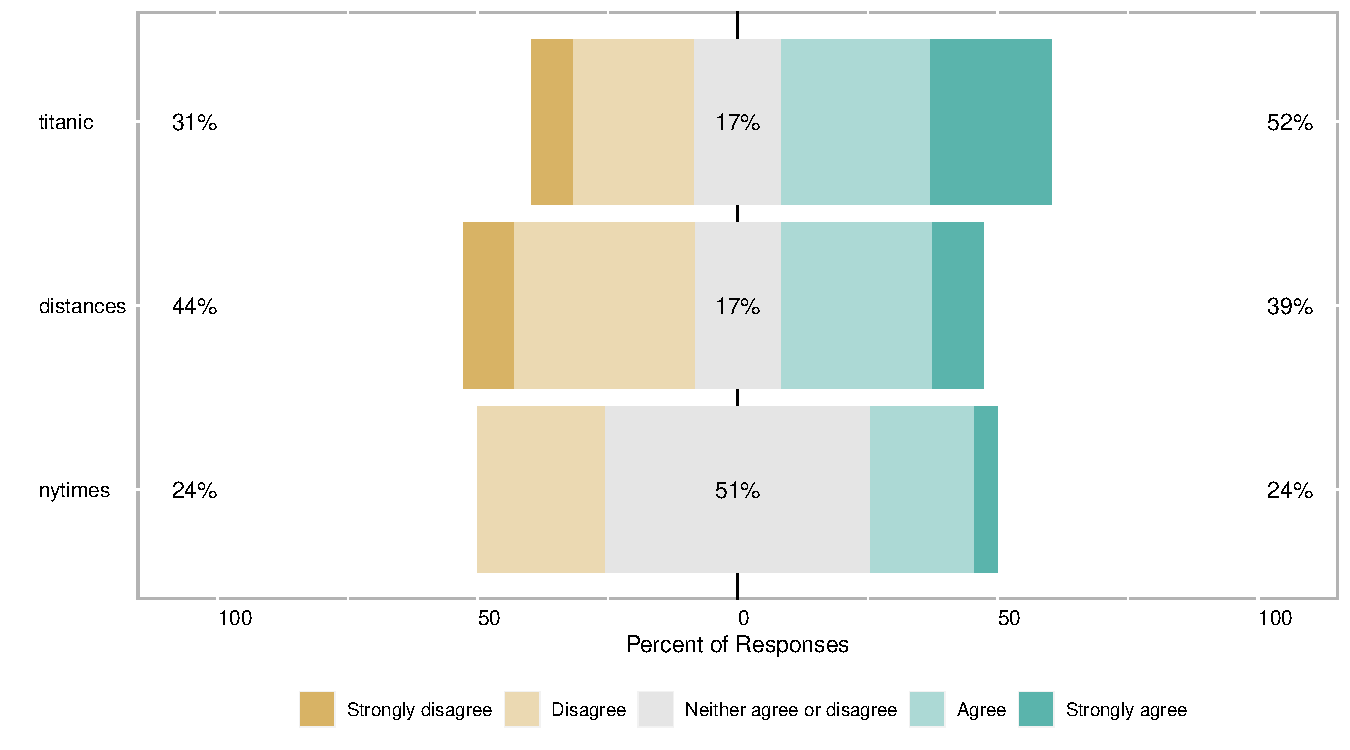
\includegraphics[width=.9\textwidth]{cp6/usefulness_overall.pdf}
    \caption{Diverging stacked plot of the usefulness of the text automatically identified for each task}
    \label{fig:usefulness-by-task}
\end{figure}


The mixed results for the \texttt{NYTimes} task might explain the lack of differences in the correctness scores observed for this task. 
Although anecdotal, one interesting feedback for this task was from a participant who described that 
their experience with the \texttt{BeautifulSoup} module influenced their negative ratings---``\textit{I have experience with BeautifulSoup and webscraping, and so my [negative] ratings of the usefulness of the highlights may have been influenced by that}''.








Surprisingly, when we look at the ratings per type of artifact (Figure~\ref{fig:usefulness-by-artifact-type}), API documents had the most useful highlights.
For this type of artifact, we observe that positive ratings originate from artifacts that follow a \textit{`how to'} format,
which is not conventional for API documents~\cite{robillard2011field, arya2020}. The highlights on Stack Overflow artifacts were also perceived as useful
and participants expressed familiarity with this type of artifact, where the highlights helped them determine parts of the page to ignore---``\textit{the highlight [on Stack Overflow] helped me quickly determine which parts of the page to ignore}''.


Miscellaneous web pages were the artifact where participants disagreed the most on the usefulness of the text automatically identified.
Due to their `\textit{tutorial}' format, these artifacts are lengthy and some participants expressed that they would like more direct explanations about how to use the modules of each task---``\textit{I have used these libraries before to some extent, so I don't need a narrative around purpose or procedure}''. 



\begin{figure}
    \centering
    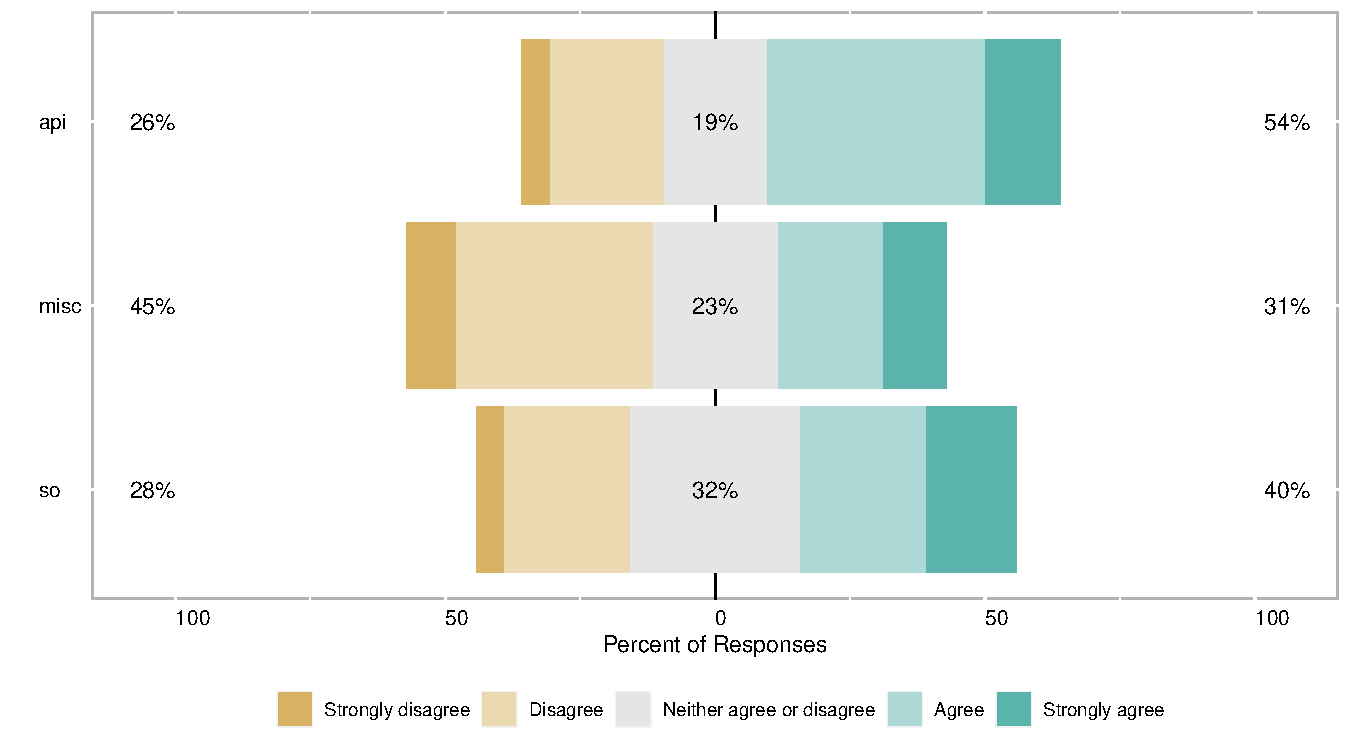
\includegraphics[width=.9\textwidth]{cp6/usefulness_per_type.pdf}
    \caption{Diverging stacked plot of the usefulness of the text automatically identified for each type of artifact}
    \label{fig:usefulness-by-artifact-type}
\end{figure}














% These artifacts follow a `\textit{tutorial}' format might be more appropriate for novices 



% ``\textit{I have used these libraries before to some extent so I don't need a narrative around purpose or procedure}''



% 




% ``\textit{When doing the second task, with the highlighted references, I was able to move much quicker. I quickly glanced at each resource, reading just the highlights to determine how valuable that resource was. The highlights allowed me to focus on the most relevant resources, gathering the necessary information to complete the task. }''









% \medskip
% \begin{small}
% \begin{bluequote}
%     ``\textit{Some of the highlights were useful when there were clear special meanings to particular function arguments like as\_index=True}''
% \end{bluequote}
% \end{small}




% \medskip
% \begin{small}
% \begin{bluequote}
%     ``\textit{I also went to the `documentation $>$ distance', but surprisingly nothing was highlighted}''
% \end{bluequote}
% \end{small}
